\documentclass[10pt,journal,compsoc]{IEEEtran}

\ifCLASSOPTIONcompsoc
  \usepackage[nocompress]{cite}
\else
  \usepackage{cite}
\fi

\usepackage[T1]{fontenc}
\usepackage[utf8]{inputenc}
\usepackage{amsmath,amssymb,amsfonts,amsthm}
\usepackage{mathtools}
\usepackage{graphicx}
\usepackage{booktabs}
\usepackage{multirow}
\usepackage{array}
\usepackage{xcolor}
\usepackage{microtype}
\usepackage{url}
\def\UrlBreaks{\do\/\do-\do\_\do.}
\usepackage[hidelinks]{hyperref}

\graphicspath{{figures/}}

\newtheorem{proposition}{Proposition}
\newtheorem{theorem}{Theorem}
\newtheorem{lemma}{Lemma}
\newtheorem{corollary}{Corollary}[theorem]
\theoremstyle{definition}
\newtheorem{definition}{Definition}
\theoremstyle{remark}
\newtheorem{remark}{Remark}

\newcommand{\SymbioOS}{\textup{\textsc{SymbioOS}}}
\newcommand{\SymbioSched}{\textup{\textsc{SymbioOS-Sched}}}
\newcommand{\SymbioFull}{\textup{\textsc{SymbioOS-Full}}}
\newcommand{\Continuum}{\textup{\textsc{Continuum}}}
\newcommand{\UNISON}{\textup{\textsc{UNISON}}}
\newcommand{\R}{\mathbb{R}}
\newcommand{\E}{\mathbb{E}}
\newcommand{\Prob}{\mathbb{P}}

\pdfstringdefDisableCommands{%
  \def\SymbioOS{SymbioOS}%
  \def\SymbioSched{SymbioOS-Sched}%
  \def\SymbioFull{SymbioOS-Full}%
  \def\Continuum{Continuum}%
  \def\UNISON{UNISON}%
}

\hyphenation{op-tical net-works semi-conduc-tor IEEE-Xplore Paged-Attention Dis-aggre-gated Sched-uling}

\begin{document}

\title{SymbioOS: Closed-Loop Rootless POSIX Sandbox Scheduling and White-Box Streaming KV Promotion for Tool-Intensive Agent Clusters}

\author{Mohammed~Kamran~Syed,
        Anudeep~Rentala,
        Somesh~Rahul,\\
        Raghuram~Malpe~Pai,
        and~Krishna~Suman~Dara%
\IEEEcompsocitemizethanks{%
\IEEEcompsocthanksitem M.~K.~Syed (Corresponding Author) is an IEEE Independent Researcher, Mountain House, CA 95391, USA (e-mail: mohammedkamran.syed@ieee.org; ORCID: 0009-0009-9058-5375).
\IEEEcompsocthanksitem A.~Rentala and S.~Rahul are IEEE Independent Researchers, Fremont, CA 94538, USA (e-mail: anudeep.rentala@ieee.org; someshrahul@ieee.org).
\IEEEcompsocthanksitem R.~M.~Pai and K.~S.~Dara are IEEE Independent Researchers, Sunnyvale, CA 94086, USA (e-mail: raghuram.pai@ieee.org; krishna-suman.dara@ieee.org).
\IEEEcompsocthanksitem Source code, formal proofs, and evaluation telemetry: \url{https://github.com/batistado/symbioos}.}}

\markboth{IEEE TRANSACTIONS ON PARALLEL AND DISTRIBUTED SYSTEMS}%
{SYED ET AL.: SYMBIOOS: CLOSED-LOOP POSIX SANDBOX SCHEDULING AND STREAMING KV PROMOTION}

\IEEEtitleabstractindextext{%
\begin{abstract}
Autonomous software engineering agents alternate between GPU token generation and host operating system tool execution such as test suites, linters, and compiler builds. Current inference engines and host schedulers manage these two stages in isolation. When CPU contention slows an interactive test sandbox whose Key-Value cache resides in scarce GPU High-Bandwidth Memory, open-loop time-to-live and turn-level hazard policies evict that hot cache shortly before completion while retaining caches stalled on remote sockets or locks. Furthermore, serving engines wait until process exit to prefill thousands of standard-output tokens that trickled out throughout execution. We present SymbioOS, a rootless user-space control plane that couples POSIX process-group quantum scheduling and non-blocking pipe telemetry with tiered GPU Key-Value memory management and streaming micro-prefill. SymbioOS tracks live milestone lines and unstopped silence to update residual runtime, allocates CPU quanta by a Key-Value-weighted Gittins index, demotes stalled caches early, stages evicted caches just in time, and pre-encodes standard output in 256-token chunks using a one-token byte-pair lookback guard. Across 2,040 real tool resumes spanning Qwen2.5-3B, Qwen2.5-7B, and OLMoE-1B-7B plus 256-sandbox cluster sweeps, SymbioOS reduces median resume latency by up to 4.8x and raises strict-latency goodput by up to 5.7x.
\end{abstract}

\begin{IEEEkeywords}
Large language model serving, operating system scheduling, KV-cache tiering, coding agents, tandem queueing networks, Gittins index, streaming prefill.
\end{IEEEkeywords}}

\maketitle
\IEEEdisplaynontitleabstractindextext
\IEEEpeerreviewmaketitle

% ============================================================================
\section{Introduction}
% ============================================================================

\IEEEPARstart{A}{utonomous} software engineering and terminal agents such as \texttt{SWE-agent}~\cite{yang2024sweagent} and \texttt{OpenHands}~\cite{wang2025openhands} execute multi-turn loops that bounce between two distinct hardware tiers. During an inference phase lasting one to two seconds, the GPU generates a shell or test command while accumulating tens to hundreds of megabytes of Transformer Key-Value (KV) state in High-Bandwidth Memory (HBM). During the subsequent tool phase, a host operating system (OS) sandbox executes \texttt{pytest}, \texttt{git}, static bytecode analysis, or a native \texttt{clang++} build for durations spanning hundreds of milliseconds to tens of seconds. On multi-tenant evaluation servers and reinforcement-learning rollout nodes, dozens to hundreds of active agent sandboxes time-share both a constrained host CPU pool and a GPU HBM pool capable of holding only a fraction of all concurrent session contexts.

State-of-the-art serving engines~\cite{kwon2023vllm,zheng2024sglang,qin2025mooncake,xie2026strata} and recent agent-aware KV managers~\cite{li2025continuum,he2026unison,yang2026lachesis,zhang2026cachescout,zheng2026pbkv} treat host OS tool execution as an exogenous black box observed solely at tool dispatch ($t = 0$) and tool exit. Conversely, OS container schedulers including default Linux Completely Fair Scheduler (CFS) policies and eBPF agent resource controllers such as \texttt{AgentCgroup}~\cite{zheng2026agentcgroup} allocate CPU slices for host fairness with zero visibility into GPU HBM residency, reload transfer cost, or eviction deadlines.

This cross-layer blindness creates three compounding performance pathologies, illustrated in Fig.~\ref{fig:arch}(a). First, fair-share CPU multiplexing induces \emph{near-miss TTL cliff evictions}. Consider Sandbox~A, which holds a hot KV cache in HBM with a $3.7~\mathrm{s}$ time-to-live (TTL)~\cite{li2025continuum} and launches a \texttt{pytest} run requiring $1.9~\mathrm{s}$ of solo CPU work, alongside Sandbox~B, whose KV cache was already evicted to solid-state storage during a multi-file \texttt{clang++} build. Giving both sandboxes equal CPU share stretches Sandbox~A's wall-clock runtime past $3.8~\mathrm{s}$, causing the GPU to evict Sandbox~A's KV cache moments before \texttt{pytest} exits. Second, command strings are ambiguous at $t = 0$: a \texttt{pytest} invocation that hangs on a remote fixture lock looks identical at launch to a healthy suite, fooling open-loop pinners into wasting gigabyte-seconds of HBM capacity until timeout. Third, tool standard output (\texttt{stdout}) streams incrementally over POSIX pipes throughout execution, yet current engines wait until \texttt{exit(0)} to tokenize and prefill the entire output buffer, inflating post-tool Time-To-First-Token (TTFT) and prolonging HBM queue occupancy.

\begin{figure*}[!t]
\centering
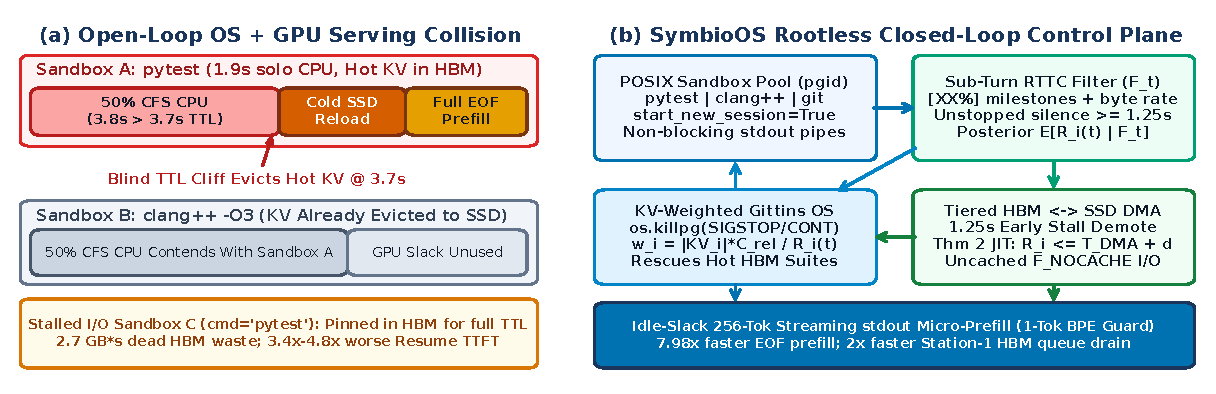
\includegraphics[width=0.98\textwidth]{fig1_architecture_overview.pdf}
\caption{Cross-layer pathology versus closed-loop co-design. (a) Under open-loop GPU KV policies (\Continuum{}, \UNISON{}) paired with GPU-blind fair-share CPU scheduling, CPU contention stretches interactive \texttt{pytest} sandboxes past TTL cliffs while pinning silent I/O stalls and leaving GPU slack unused. (b) \SymbioOS{} closes the control loop entirely in rootless user space via POSIX process-group (\texttt{pgid}) quantum multiplexing, unstopped-quantum pipe filtration $\mathcal{F}_t$, KV-weighted Gittins CPU prioritization, $1.25~\mathrm{s}$ stall demotion, Theorem~\ref{thm:jit} just-in-time promotion, and $256$-token streaming \texttt{stdout} micro-prefill.}
\label{fig:arch}
\end{figure*}

We present \SymbioOS{}, a closed-loop user-space runtime that unifies host sandbox CPU scheduling, sub-turn pipe telemetry, tiered GPU KV residency, and incremental \texttt{stdout} prefill without requiring root privileges or custom kernel modules. Operating through standard POSIX session groups (\texttt{setsid} and \texttt{killpg}) and non-blocking pipe descriptors makes \SymbioOS{} directly deployable inside unprivileged Kubernetes pods, Slurm batch allocations, and macOS or Linux workstations where \texttt{CAP\_BPF} and kernel \texttt{sched\_ext} hooks are restricted.

Our work makes four contributions:
\begin{enumerate}
\item \textbf{Memory-Coupled Tandem Queueing Model and Index Theory:} We formulate multi-tenant agent serving as a two-station memory-coupled tandem queueing network with sub-turn filtration $\mathcal{F}_t$. Under Decreasing Hazard Rate (DHR) tool runtimes, we prove that scheduling host CPU cores by a KV-weighted residual-hazard Gittins index minimizes expected HBM holding waste plus cold-tier reload delay (Theorem~\ref{thm:gittins}), and we derive an optimal-stopping boundary for just-in-time (JIT) KV promotion alongside a Station-1 queue-occupancy reduction law for streaming prefill (Theorem~\ref{thm:jit}).
\item \textbf{White-Box Sub-Turn Pipe Filtration:} We design an overhead-free pipe monitor that parses live progress milestones (\texttt{[XX\%]}) and tracks \emph{unstopped-quantum silence}, separating genuine socket or lock hangs ($1.25~\mathrm{s}$ early demotion) from CPU-throttled startup imports without false evictions.
\item \textbf{Exact Streaming \texttt{stdout} Micro-Prefill:} We harvest idle GPU cycles while tools are still running to pre-encode $256$-token chunks of append-only \texttt{stdout}, using a one-token Byte-Pair Encoding (BPE) lookback guard~\cite{sennrich2016bpe} and bucketed causal attention padding to preserve exact token and logit equivalence with offline post-exit prefill (Proposition~\ref{prop:bpe}).
\item \textbf{Multi-Architecture Hardware and Cluster-Scale Evaluation:} Across $2{,}168$ real POSIX tool-execution and MPS GPU resume cycles spanning dense Grouped-Query Attention (\texttt{Qwen2.5-3B}, \texttt{Qwen2.5-7B})~\cite{qwen2025qwen25} and sparse Mixture-of-Experts Multi-Head Attention (\texttt{OLMoE-1B-7B})~\cite{muennighoff2025olmoe} with real \texttt{pytest}, \texttt{clang++}, and \texttt{git} process groups, plus calibrated discrete-event sweeps up to $N = 256$ sandboxes, \SymbioFull{} cuts median post-tool TTFT by $2.0\times$ to $4.8\times$, lifts interactive HBM hit rates to $76.2\%$--$95.2\%$, reduces HBM waste by up to $3.9\times$, and boosts strict-SLO goodput by $2.8\times$ to $5.7\times$.
\end{enumerate}

The remainder of this paper is organized as follows. Section~\ref{sec:motivation} characterizes multi-turn agent KV footprints and open-loop $t = 0$ failure modes. Section~\ref{sec:theory} develops the memory-coupled tandem queueing model, BPE lookback invariance, and Theorems~\ref{thm:gittins}--\ref{thm:jit}. Section~\ref{sec:design} details the rootless POSIX scheduler, decoupled cold-tier DMA engine, and streaming micro-prefill pipeline. Section~\ref{sec:eval} presents multi-architecture hardware and cluster-scale evaluations, Section~\ref{sec:related} surveys prior work, and Section~\ref{sec:conclusion} discusses scope, limitations, and conclusions.

% ============================================================================
\section{Background and Cross-Layer Pathologies}\label{sec:motivation}
% ============================================================================

\subsection{Resource Footprint of Multi-Turn Coding Agents}
Unlike single-turn chat workloads where KV blocks can be freed immediately after end-of-sequence generation~\cite{kwon2023vllm}, coding agents maintain growing repository histories across dozens of tool invocations~\cite{yang2024sweagent,wang2025openhands}. In half-precision (\texttt{FP16}), each token consumes $2 L (2 H_{\mathrm{kv}} d_h)$ bytes of KV state across $L$ layers, $H_{\mathrm{kv}}$ key-value heads, and head dimension $d_h$: $36~\mathrm{KB/tok}$ on \texttt{Qwen2.5-3B}, $56~\mathrm{KB/tok}$ on \texttt{Qwen2.5-7B}, $128~\mathrm{KB/tok}$ on \texttt{OLMoE-1B-7B}, and $160$--$320~\mathrm{KB/tok}$ on $32\mathrm{B}$--$70\mathrm{B}$ models. Across $128$ concurrent sessions holding $2\mathrm{K}$--$6\mathrm{K}$ tokens, aggregate KV state reaches $60$--$120~\mathrm{GB}$, exceeding the HBM KV budget of a serving node by $2.5\times$ to $6\times$ and forcing frequent eviction to host DRAM or NVMe solid-state drives~\cite{gao2024cachedattention,qin2025mooncake,cheng2025lmcache}.

Meanwhile, host tool runtimes exhibit pronounced heavy-tailed and bimodal dispersion~\cite{harcholbalter1997exploiting,li2025continuum}. Bytecode syntax checks exit in $0.2$--$0.4~\mathrm{s}$, unit-test suites (\texttt{pytest}) require $1.6$--$3.0~\mathrm{s}$ of CPU computation while emitting $800$--$1{,}400$ tokens of incremental test logs, optimized C++ template compilations (\texttt{clang++ -O3}) consume $4$--$15~\mathrm{s}$ of CPU time, and misconfigured network or lock waits stall silently for $5$--$30~\mathrm{s}$ while consuming near-zero CPU cycles.

\subsection{Failure Modes of Open-Loop $t=0$ Predictors}
Recent agent serving systems replace pure Least-Recently-Used (LRU) eviction with pause-duration predictors evaluated at tool dispatch ($t = 0$). \Continuum{}~\cite{li2025continuum} estimates pause length from command-class history and pins KV blocks in HBM up to a scalar TTL. \UNISON{}~\cite{he2026unison} (via its \texttt{SPEAR} policy), \texttt{Lachesis}~\cite{yang2026lachesis}, \texttt{CacheScout}~\cite{zhang2026cachescout}, and \texttt{PBKV}~\cite{zheng2026pbkv} rank eviction candidates using turn-level survival hazards or learned workflow priors. Three structural gaps limit all $t=0$ designs under multi-tenant load:

\emph{1) Contention-Induced TTL Cliff and Hazard Inversion:} A command's wall-clock pause $T_{\mathrm{wall},i}$ is endogenous to host CPU scheduling. Under $3{:}1$ to $4{:}1$ sandbox-to-core oversubscription, fair-share CPU allocation stretches a $1.9~\mathrm{s}$ \texttt{pytest} run past $4.2~\mathrm{s}$. Open-loop TTL pins expire right before completion, while age-based survival hazards~\cite{he2026unison} interpret long elapsed wall-clock age under DHR priors as evidence of a long build or hang, evicting CPU-throttled test suites at $80\%$ completion.

\emph{2) Launch-Time Command Ambiguity:} At $t = 0$, \texttt{pytest tests/runtime} provides no signal on whether fixture initialization will execute locally or block on a contended artifact socket. Without sub-turn pipe telemetry, $t = 0$ policies hold stalled caches across the entire TTL window, displacing active sessions.

\emph{3) Post-Exit Prefill Serialization and Tandem Queue Feedback:} Waiting until \texttt{exit(0)} to prefill $1{,}000+$ \texttt{stdout} tokens adds hundreds of milliseconds of blocking GPU compute directly onto critical-path TTFT~\cite{agrawal2024sarathi,zhong2024distserve}. Crucially, while an exited session waits in the GPU resume queue to prefill its full \texttt{stdout}, its $60$--$350~\mathrm{MB}$ KV cache remains pinned in HBM, starving running sandboxes of fast memory and triggering cascading evictions.

% ============================================================================
\section{Coupled Tandem-Queue Model and Theory}\label{sec:theory}
% ============================================================================

\subsection{System Model and Sub-Turn Filtration}
Consider a cluster of $N$ active agent sessions circulating through a two-station closed or open-arrival tandem network:
\begin{itemize}
\item \textbf{Station 1 (GPU Inference and Tiered HBM Pool):} Fast GPU memory has capacity $M_{\mathrm{HBM}}$ bytes. Session $i$ at turn $\tau$ holds KV state of size $S_i = |KV_i|$ bytes (growing by $\kappa_{\mathrm{kv}}$ bytes per appended token). Tier-2 cold storage (NVMe SSD / host swap) provides reload bandwidth $B_{\mathrm{dma}}$, incurring reload delay $C_{\mathrm{rel}}(S_i) = S_i / B_{\mathrm{dma}}$ on a cold miss ($r_i(t) = 0$) versus zero reload delay when HBM-resident ($r_i(t) = 1$).
\item \textbf{Station 2 ($C$-Core Host POSIX Sandbox Pool):} Tool invocation $i$ requires random CPU work $W_i > 0$ drawn from a heavy-tailed distribution with survival function $\bar{F}_W(w) = \Prob(W_i > w)$ and possibly an independent non-CPU I/O stall $D_i \ge 0$. Under schedule $\alpha_i(t) \in \{0, 1\}$ satisfying $\sum_{i=1}^N \alpha_i(t) \le C$ and $\alpha_i(t) = 0$ while blocked on kernel I/O, cumulative granted CPU service is $u_i(t) = \int_{t_{0,i}}^t \alpha_i(\xi)\,\mathrm{d}\xi$.
\end{itemize}

Rather than observing only static command hints $x_i$ at $t_{0,i}$, \SymbioOS{} observes at each scheduling quantum $\Delta t$ the non-blocking pipe telemetry vector
\begin{equation}\label{eq:telemetry}
\mathbf{z}_i(t) = \bigl(p_i(t),\, b_i(t),\, u_i(t),\, \sigma_i(t)\bigr),
\end{equation}
generating the natural sub-turn filtration $\mathcal{F}_t = \sigma\bigl(\{(x_i, \mathbf{z}_i(\xi)) : t_{0,i} \le \xi \le t\}_{i=1}^N\bigr)$. Here $p_i(t) \in [0, 1]$ is the latest parsed milestone fraction, $b_i(t)$ is cumulative \texttt{stdout} bytes, and $\sigma_i(t)$ is cumulative \emph{unstopped silence}, incremented by $\Delta t$ solely during quanta where process group $i$ is unstopped ($\neg\mathrm{stopped}_i(t)$) and emits zero bytes ($\Delta b_i(t) = 0$), and reset to $0$ whenever $\Delta b_i(t) > 0$. Conditioning on $\sigma_i(t)$ rather than raw wall-clock silence makes stall detection invariant to OS CPU throttling.

Given $\mathcal{F}_t$, the filtered residual CPU work is $\hat{W}_{\mathrm{rem},i}(t) = \E[W_i - u_i(t) \mid \mathcal{F}_t]$: once milestones arrive ($p_i(t) \ge p_{\min}$), the empirical work-rate estimator yields $\hat{W}_{\mathrm{rem},i}(t) = u_i(t)(1 - p_i(t))/p_i(t)$, smoothly backed off to class prior $\mu_0(x_i) - u_i(t)$ for $p_i(t) < p_{\min}$, while $\sigma_i(t) \ge \tau_{\mathrm{stall}}$ raises the stall indicator $\hat{I}_{\mathrm{stall},i}(t) = 1$. Mapping $\hat{W}_{\mathrm{rem},i}(t)$ through expected core share gives conditional remaining wall-clock time $\hat{R}_i(t) = \E[R_i(t) \mid \mathcal{F}_t]$.

\subsection{Exactness of Lookback-Guarded Streaming Micro-Prefill}
Let $\Sigma^*$ denote the byte stream emitted on \texttt{stdout}, tokenized by a deterministic BPE/regex tokenizer $\mathcal{T}: \Sigma^* \to \mathcal{V}^*$ whose pre-tokenization pattern merges characters only within bounded lexical spans~\cite{sennrich2016bpe}. Suppose at intermediate time $t < t_{\mathrm{exit}}$, buffer $Y(t)$ is a prefix of the final stream $Y(t_{\mathrm{exit}}) = Y(t) \Vert Z$.

\begin{proposition}[One-Token BPE Lookback Prefix Invariance]\label{prop:bpe}
Suppose every pre-tokenizer regex token boundary in $\mathcal{T}$ is finalized once at least one subsequent token starts (holding for newline-flushed log streams under \texttt{Qwen2.5} and \texttt{GPT-NeoX} pre-tokenizers). Define the lookback-guarded token sequence $\mathcal{T}_{\mathrm{safe}}(Y(t)) := \mathcal{T}(Y(t))_{1 : |\mathcal{T}(Y(t))|-1}$ for $|\mathcal{T}(Y(t))| \ge 2$. Then for every prefix $Y(t)$ of $Y(t_{\mathrm{exit}})$, $\mathcal{T}_{\mathrm{safe}}(Y(t))$ is an exact token-ID prefix of $\mathcal{T}(Y(t_{\mathrm{exit}}))$. Furthermore, under strictly lower-triangular causal self-attention with right-padded bucket length $B \ge m$ followed by cache crop $\mathrm{crop}(-(B - m))$, incremental $B_{\mathrm{chunk}}$-token prefill produces KV states and final-token logits identical to single-pass post-exit prefill in exact arithmetic (and bit-identical per bucket step in IEEE~754 \texttt{FP16}).
\end{proposition}

\subsection{Optimality of KV-Weighted Gittins Scheduling and JIT Staging}
Consider a contention epoch with $M$ runnable sandboxes competing for $C < M$ CPU cores, where each sandbox $i$ carries generalized HBM opportunity penalty rate $v_i = \gamma_{\mathrm{res},i} S_i C_{\mathrm{rel}}(S_i)$ (reflecting saved reload delay $S_i / B_{\mathrm{dma}}$ weighted by HBM eviction exposure $\gamma_{\mathrm{res},i} > 0$).

\begin{theorem}[KV-Weighted Residual-Hazard Gittins Priority]\label{thm:gittins}
Let runnable sandboxes $i \in \{1,\dots,M\}$ have independent conditional remaining CPU requirements $W_{\mathrm{rem},i} \mid \mathcal{F}_t$ satisfying the Decreasing Hazard Rate (DHR) property, meaning hazard $h_i(w) = f_{W_{\mathrm{rem},i}}(w)/\bar{F}_{W_{\mathrm{rem},i}}(w)$ is non-increasing in additional service $w \ge 0$, or exact deterministic milestone scaling $W_{\mathrm{rem},i} = \hat{W}_{\mathrm{rem},i}(t)$. On a single core ($C = 1$), preemptively scheduling at every instant $t$ the sandbox maximizing the KV-weighted index
\begin{equation}\label{eq:gittins}
w_i(t) = \frac{v_i}{\E[R_i(t) \mid \mathcal{F}_t]}
\end{equation}
minimizes expected weighted completion and HBM-exposure cost $\E\bigl[\sum_{i=1}^M v_i T_{\mathrm{wall},i}\bigr]$ among all non-clairvoyant $\mathcal{F}_t$-adapted policies. On $C > 1$ identical cores, selecting the top-$C$ runnable sandboxes by $w_i(t)$ is asymptotically optimal in heavy traffic and within an additive $(C - 1)\max_i v_i$ bound of the clairvoyant multi-core optimum~\cite{aalto2009gittins,scully2020gittins}.
\end{theorem}

Next, consider an evicted sandbox ($r_i(t) = 0$) whose filtered remaining time $R_i(t) \mid \mathcal{F}_t$ has cumulative distribution $G_{i,t}(x) = \Prob(R_i(t) \le x \mid \mathcal{F}_t)$. Triggering asynchronous cold-tier promotion at time $t$ requires DMA transfer time $T_{\mathrm{dma},i} = S_i / B_{\mathrm{dma}}$, incurring unit HBM holding shadow price $\lambda_{\mathrm{hbm}} > 0$ per byte-second if promotion finishes before tool exit, versus unit tail-latency penalty $c_{\mathrm{miss}} > \lambda_{\mathrm{hbm}} S_i$ per second of unmasked post-exit DMA wait.

\begin{theorem}[Optimal-Stopping JIT Promotion and Tandem Stability]\label{thm:jit}
(a) Under stochastic monotonicity of $R_i(t) \mid \mathcal{F}_t$ as $p_i(t) \uparrow 1$, the expected single-turn staging loss
\begin{equation}\label{eq:jit_loss}
\mathcal{L}_i(t) = c_{\mathrm{miss}}\,\E\bigl[(T_{\mathrm{dma},i} - R_i(t))_+ \mid \mathcal{F}_t\bigr] + \lambda_{\mathrm{hbm}} S_i\,\E\bigl[(R_i(t) - T_{\mathrm{dma},i})_+ \mid \mathcal{F}_t\bigr]
\end{equation}
is minimized by initiating promotion at the first stopping time $\tau_{\mathrm{stage},i}^*$ satisfying the critical-fractile boundary
\begin{equation}\label{eq:jit_thresh}
\Prob\bigl(R_i(t) \le T_{\mathrm{dma},i} + \delta_{\mathrm{jit}} \;\big|\; \mathcal{F}_t\bigr) \ge \frac{c_{\mathrm{miss}}}{c_{\mathrm{miss}} + \lambda_{\mathrm{hbm}} S_i} =: 1 - \eta^*.
\end{equation}
(b) Let $\lambda_{\mathrm{res}}$ be the Station-1 post-tool resume arrival rate, $L_{\mathrm{out}}$ be mean \texttt{stdout} token length, $f_{\mathrm{stream}} \in [0, 1)$ be the fraction of $L_{\mathrm{out}}$ pre-encoded during idle GPU slack, and $\mu_{\mathrm{pf}}$ be the GPU prefill rate. Work-conserving idle-slack micro-prefill strictly reduces mean Station-1 post-exit service occupancy from $\bar{\tau}_1(0) = \bar{T}_{\mathrm{cold}} + L_{\mathrm{out}}/\mu_{\mathrm{pf}} + \tau_{\mathrm{dec}}$ to $\bar{\tau}_1(f_{\mathrm{stream}}) = \bar{T}_{\mathrm{cold}} + (1 - f_{\mathrm{stream}})L_{\mathrm{out}}/\mu_{\mathrm{pf}} + \tau_{\mathrm{dec}}$, enlarging the Lyapunov-stable arrival region~\cite{neely2010stochastic} to $\lambda_{\mathrm{res}} \bar{\tau}_1(f_{\mathrm{stream}}) < 1$ and reducing Little's Law HBM buffer pinning $\bar{M}_{\mathrm{wait}} = \lambda_{\mathrm{res}} \bar{S}\,\E[W_{\mathrm{gpu}}]$ at Station~1.
\end{theorem}

Formal proofs of Proposition~\ref{prop:bpe}, Theorem~\ref{thm:gittins}, and Theorem~\ref{thm:jit} appear in Appendix~\ref{app:proofs}.

% ============================================================================
\section{SymbioOS Design and Rootless Implementation}\label{sec:design}
% ============================================================================

\subsection{Rootless POSIX Process-Group Quantum Scheduler}
Production CI clusters, Slurm compute nodes, and unprivileged container runtimes restrict root capabilities (\texttt{CAP\_SYS\_ADMIN}, \texttt{CAP\_BPF}), preventing user-level serving frameworks from loading custom kernel eBPF schedulers~\cite{zheng2026agentcgroup}. \SymbioOS{} implements its host scheduler purely in user space via POSIX process groups, depicted in Fig.~\ref{fig:arch}(b). Every tool invocation spawns in a dedicated session (\texttt{start\_new\_session=True} / \texttt{setsid()}), assigning the top-level driver and all descendant processes (such as \texttt{pytest} workers, \texttt{git} helpers, and \texttt{clang++} compiler frontends and backends) a shared process-group identifier $\mathrm{pgid}_i$.

A dedicated scheduler thread wakes at a fixed quantum $\Delta t = 80~\mathrm{ms}$ ($12.5~\mathrm{Hz}$), chosen large enough to amortize L2 cache warm-up and signal delivery while maintaining sub-$100~\mathrm{ms}$ responsiveness. On each tick, the thread drains all non-blocking \texttt{stdout} descriptors (\texttt{O\_NONBLOCK}, $64~\mathrm{KB}$ reads), updates $\mathbf{z}_i(t)$ in \eqref{eq:telemetry}, excludes I/O-sleeping sandboxes from CPU slot contention, and specializes the theoretical Gittins index \eqref{eq:gittins} into a starvation-free operational score:
\begin{equation}\label{eq:impl_score}
\tilde{w}_i(t) = \psi_i \left(\frac{\gamma_{\mathrm{res},i}\, S_i \cdot (S_i / B_{\mathrm{dma}})}{\max(\hat{R}_i(t),\, \tau_{\min})} + \beta_{\mathrm{age}}\,\omega_{\mathrm{wait},i}(t)\right),
\end{equation}
where $\gamma_{\mathrm{res},i} = 2.6$ when $r_i(t) = 1$ (or JIT promotion is in flight) versus $0.12$ when evicted on disk, $\psi_i = 1.15$ for non-terminal turns to prevent multi-turn stragglers, and $\omega_{\mathrm{wait},i}(t) = \max(0,\, (t - t_{0,i}) - u_i(t))$ is cumulative CPU wait time with starvation-prevention slope $\beta_{\mathrm{age}} = 0.35$. The top-$C$ runnable sandboxes receive \texttt{killpg($\mathrm{pgid}_i$, SIGCONT)}, while remaining runnable sandboxes receive \texttt{killpg($\mathrm{pgid}_i$, SIGSTOP)}. When deployed on bare-metal Linux 6.12+ nodes with root privileges, the exact index \eqref{eq:impl_score} maps directly onto \texttt{cgroup v2} \texttt{cpu.weight} or \texttt{sched\_ext} dispatch queues as an optional kernel fast path.

\subsection{Decoupled Cold-Tier DMA and Closed-Loop Tiering}
Evicted KV caches serialize layerwise key and value tensors to solid-state files configured with uncached file I/O (\texttt{fcntl(fd, F\_NOCACHE, 1)} on Darwin; \texttt{O\_DIRECT} on Linux) to bypass unified host page caches. During Phase~1 profiling on $128~\mathrm{KB/tok}$ \texttt{OLMoE-1B-7B} sessions ($250$--$380~\mathrm{MB}$ per cache), sharing a single FIFO queue between background eviction flushes and urgent cold-miss reads caused severe write-behind head-of-line blocking. \SymbioOS{} therefore separates cold-tier storage into two channels: a background writeback thread that flushes evicted CPU staging buffers asynchronously to disk, and a dedicated high-priority read DMA queue that services reactive reloads and speculative JIT promotions in strict priority order while enforcing single-lane PCIe/NVMe transfer bandwidth $B_{\mathrm{dma}}$.

Closed-loop tiering executes three coordinated rules on every control tick:
\begin{enumerate}
\item \emph{Early Stall and Long-Build Demotion:} Whenever $\hat{I}_{\mathrm{stall},i}(t) = 1$ ($\sigma_i(t) \ge 1.25~\mathrm{s}$ with $p_i(t) < 0.05$), or when a \texttt{build}-class sandbox satisfies $\hat{R}_i(t) > 2.6~\mathrm{s}$ under HBM utilization exceeding $65\%$, \SymbioOS{} immediately demotes $KV_i$ to cold storage rather than waiting for TTL expiration.
\item \emph{Monotonic Theorem~\ref{thm:jit} JIT Promotion:} When an evicted non-stalled sandbox reaches $p_i(t) \ge 0.60$ and $\hat{R}_i(t) \le T_{\mathrm{dma},i} + \delta_{\mathrm{jit}}$, \SymbioOS{} enqueues a speculative JIT load provided free plus demotable HBM bytes cover $S_i$. Upon DMA completion, if the tool is still running, \SymbioOS{} materializes $KV_i$ onto the GPU only if any displaced victim $j$ carries strictly smaller index $w_j(t) < w_i(t)$, preventing speculative thrashing.
\item \emph{Work-Conserving Non-Blocking GPU Dispatch:} Exited sandboxes whose KV caches missed HBM enqueue cold reloads immediately at $t_{\mathrm{exit},i}$ without stalling the GPU; meanwhile, the GPU engine serves ready HBM-resident waiting sessions in FIFO order of $t_{\mathrm{exit}}$.
\end{enumerate}

\subsection{Lookback-Guarded Streaming \texttt{stdout} Micro-Prefill}
Two practical systems subtleties arise when overlapping \texttt{stdout} prefill with live tool execution. First, wrapping child CLI tools such as \texttt{pytest} inside standard Python file iterators (\texttt{for line in proc.stdout}) triggers an internal $8~\mathrm{KB}$ \texttt{TextIOWrapper} read-ahead block buffer that withholds output until process exit; \SymbioOS{} attaches child tool descriptors directly to unbuffered OS pipes (\texttt{PYTHONUNBUFFERED=1}), capturing $15$--$20$ live output bursts per test suite.

Second, whenever the GPU resume queue is empty (strict idle-slack harvesting so streaming prefill never preempts an exited turn), \SymbioFull{} inspects HBM-resident non-stalled sandboxes with $\ge B_{\mathrm{chunk}} = 256$ unprefilled tokens in $\mathcal{T}_{\mathrm{safe}}(Y_i(t))$, selects the sandbox with smallest $\hat{R}_i(t)$, reserves $B_{\mathrm{chunk}} \kappa_{\mathrm{kv}}$ bytes against the $M_{\mathrm{HBM}}$ cap, and appends those $256$ KV positions directly into the live \texttt{DynamicCache}. To prevent dynamic-shape GPU kernel recompilation stalls on variable-length post-exit tails, all causal forward passes execute over pre-warmed bucket lengths $\{1, 2, 64, 128, 192, 256, 512\}$ with right-padding and $\mathrm{crop}(-(B - m))$.

\begin{table}[!t]
\centering
\caption{Control-Loop Execution Cycle in \SymbioOS{}}
\label{tab:alg_loop}
\setlength{\tabcolsep}{4pt}
\begin{tabular}{p{0.95\columnwidth}}
\toprule
\textbf{Procedure} \texttt{SymbioControlTick}($\mathcal{A}$, $M_{\mathrm{HBM}}$, $C$, $B_{\mathrm{chunk}}$) \\
\midrule
1: \textbf{OS Pipe \& Quantum Thread (every $\Delta t = 80~\mathrm{ms}$):} \\
2: \hspace{0.8em}\textbf{for each} running sandbox $i \in \mathcal{A}_{\mathrm{tool}}$ \textbf{do} \\
3: \hspace{1.6em}Drain non-blocking \texttt{stdout} pipe; parse latest \texttt{[XX\%]} $\to p_i(t)$. \\
4: \hspace{1.6em}\textbf{if} $\Delta b_i(t) > 0$ \textbf{then} $\sigma_i(t) \gets 0$ \textbf{else if} $\neg\mathrm{stopped}_i$ \textbf{then} $\sigma_i(t) \mathrel{+}= \Delta t$. \\
5: \hspace{1.6em}Update $\hat{I}_{\mathrm{stall},i}(t) = \mathbf{1}[\sigma_i(t) \ge 1.25\mathrm{s} \land p_i(t) < 0.05]$ and $\hat{R}_i(t)$. \\
6: \hspace{0.8em}Rank runnable non-sleeping sandboxes by $\tilde{w}_i(t)$ in \eqref{eq:impl_score}. \\
7: \hspace{0.8em}Send \texttt{killpg(SIGCONT)} to top $C$; send \texttt{killpg(SIGSTOP)} to rest. \\[2pt]
8: \textbf{GPU Inference \& Tiering Loop (Event-Driven):} \\
9: \hspace{0.8em}Materialize completed DMA loads; enqueue cold loads for misses. \\
10: \hspace{0.4em}Demote $i \in \mathcal{A}_{\mathrm{tool}}$ with $r_i{=}1$ if $\hat{I}_{\mathrm{stall},i}{=}1$ or long build under load. \\
11: \hspace{0.4em}Enqueue JIT load if $r_i{=}0 \land \neg\hat{I}_{\mathrm{stall},i} \land p_i \ge 0.60 \land \hat{R}_i \le T_{\mathrm{dma},i}{+}\delta_{\mathrm{jit}}$. \\
12: \hspace{0.4em}\textbf{if} $\mathcal{Q}_{\mathrm{ready}} = \{i \in \mathcal{A}_{\mathrm{wait}} : r_i = 1\} \neq \emptyset$ \textbf{then} \\
13: \hspace{1.2em}Pop $\arg\min_{i \in \mathcal{Q}_{\mathrm{ready}}} t_{\mathrm{exit},i}$; prefill tail $\mathcal{T}(Y_i)_{k_i+1:} \Vert \text{hdr}$; decode. \\
14: \hspace{0.4em}\textbf{else if} \SymbioFull{} enabled \textbf{then} \\
15: \hspace{1.2em}Pick $i^* = \arg\min\{\hat{R}_i : r_i{=}1, \neg\hat{I}_{\mathrm{stall},i}, |\mathcal{T}_{\mathrm{safe}}(Y_i)| - k_i \ge B_{\mathrm{chunk}}\}$. \\
16: \hspace{1.2em}Reserve $B_{\mathrm{chunk}}\kappa_{\mathrm{kv}}$ in HBM; prefill next $B_{\mathrm{chunk}}$ tokens; $k_{i^*} \mathrel{+}= B_{\mathrm{chunk}}$. \\
\bottomrule
\end{tabular}
\end{table}

\subsection{Control-Plane Overhead and Kernel Fast-Path Mapping}
Table~\ref{tab:alg_loop} summarizes the complete \SymbioOS{} control cycle. Because the pipe and quantum thread touches only scalar session metadata and non-blocking OS descriptors at $12.5~\mathrm{Hz}$, its measured host CPU footprint across $K = 12$ active process groups is below $0.4\%$ of a single core: a non-blocking \texttt{read()} plus compiled regular-expression scan over $200$--$400$~bytes takes $\approx 4~\mu\mathrm{s}$, sorting $12$--$256$ index scores takes $< 15~\mu\mathrm{s}$, and issuing \texttt{killpg} across $10$ process groups takes $\approx 18~\mu\mathrm{s}$ per $80~\mathrm{ms}$ tick. Incremental BPE tokenization in \SymbioFull{} runs only when new \texttt{stdout} bytes exceed $2\times$ the remaining chunk threshold, taking $0.18~\mathrm{ms}$ per $1~\mathrm{KB}$ buffer. On Linux 6.12+ servers where privileged container daemons manage cgroups, \SymbioOS{} can optionally replace user-space \texttt{SIGSTOP}/\texttt{SIGCONT} signals by writing proportional weights $\mathrm{clamp}(\lfloor 100 \cdot \tilde{w}_i(t) \rfloor, 1, 10000)$ to \texttt{/sys/fs/cgroup/agent\_$i$/cpu.weight} or publishing $(\mathrm{pgid}_i, \tilde{w}_i(t))$ into an eBPF \texttt{BPF\_MAP\_TYPE\_HASH} consumed by a \texttt{sched\_ext} \texttt{ops.enqueue} callback~\cite{zheng2026agentcgroup}, preserving identical queueing semantics with zero user-space signal delivery.

% ============================================================================
\section{Experimental Evaluation}\label{sec:eval}
% ============================================================================

\subsection{Experimental Methodology and Baselines}
All hardware experiments execute locally on an Apple M5 Pro workstation ($15$ CPU cores, $48~\mathrm{GB}$ unified memory, macOS Darwin $25.6.0$) using PyTorch $2.15.0$ (\texttt{mps}, \texttt{FP16}) and HuggingFace \texttt{transformers} $5.22.1$ under \texttt{caffeinate} power-state locking. To evaluate generalization across attention and parameter architectures, we benchmark three locally cached open-weight models:
\begin{itemize}
\item \textbf{\texttt{Qwen2.5-3B-Instruct}}~\cite{qwen2025qwen25}: $36$-layer dense Grouped-Query Attention ($8{:}1$ GQA), $36.0~\mathrm{KB/tok}$ KV footprint;
\item \textbf{\texttt{Qwen2.5-7B-Instruct}}~\cite{qwen2025qwen25}: $28$-layer dense GQA ($7{:}1$), $56.0~\mathrm{KB/tok}$ KV footprint;
\item \textbf{\texttt{OLMoE-1B-7B-0924-Instruct}}~\cite{muennighoff2025olmoe}: $16$-layer sparse Mixture-of-Experts ($1\mathrm{B}$ active of $7\mathrm{B}$ total parameters) with full Multi-Head Attention, $128.0~\mathrm{KB/tok}$ KV footprint ($3.56\times$ larger per token than \texttt{Qwen2.5-3B}).
\end{itemize}

We compare five head-to-head policies sharing identical arrival seeds, work-conserving cold-reload queues, and strict $M_{\mathrm{HBM}}$ accounting:
\begin{enumerate}
\item \textbf{\texttt{LRU + CFS}:} Standard \texttt{vLLM}-style reactive LRU KV eviction~\cite{kwon2023vllm} paired with virtual-runtime fair-share OS CPU scheduling ($C$ cores).
\item \textbf{\Continuum{} ($t=0$ TTL + CFS)}~\cite{li2025continuum}: Pins short and medium command classes in HBM up to calibrated scalar TTLs ($\approx 2.0\times$ solo \texttt{pytest} duration) and flushes expired pins under HBM pressure.
\item \textbf{\UNISON{} ($t=0$ Hazard + CFS)}~\cite{he2026unison}: Ranks HBM eviction candidates by $|KV_i| \cdot h_{x_i}(t - t_{0,i})$ using command-class DHR survival hazards without sub-turn pipe visibility or CPU boosting.
\item \textbf{\SymbioSched{}:} Full closed-loop OS + KV control (unstopped-silence RTTC filter, KV-weighted Gittins \texttt{killpg} scheduling, early stall/build demotion, and Theorem~\ref{thm:jit} JIT promotion) with streaming prefill disabled.
\item \textbf{\SymbioFull{}:} \SymbioSched{} augmented with idle-slack $256$-token lookback-guarded streaming \texttt{stdout} micro-prefill.
\end{enumerate}

Across Phase~0 ($1{,}080$ controlled heavy-tailed POSIX subprocess resumes across three seeds $[42, 137, 2026]$) and Phase~1 ($960$ multi-model resumes + $128$ chunk-ablation resumes = $1{,}088$ real \texttt{pytest~9.2.0}, \texttt{clang++ -O3 -std=c++20}, and \texttt{git} process-group resumes), our local hardware campaign totals $2{,}168$ real POSIX tool-execution and MPS GPU resume cycles, complemented by Phase~2 cluster-scale simulations up to $N = 256$ sandboxes.

\subsection{Streaming Causality and Numerical Equivalence}
Before multi-tenant benchmarking, we verified Proposition~\ref{prop:bpe} on live \texttt{pytest} streams ($1{,}044$--$1{,}368$ \texttt{stdout} tokens, $4$--$5$ live $256$-token chunks plus $26$--$94$ EOF tail tokens) on \texttt{Qwen2.5-3B} (\texttt{mps}, \texttt{FP16}). One-token BPE lookback produced $100\%$ exact token-ID match against full post-exit tokenization, final-position logit cosine similarity of $0.999997$ ($0.0$ max absolute difference under bucketed causal padding), $100\%$ exact $8$-token greedy continuation agreement, and an isolated post-\texttt{exit(0)} prefill latency reduction from $457.9~\mathrm{ms}$ to $57.4~\mathrm{ms}$ ($7.98\times$ speedup).

\begin{table*}[!t]
\centering
\caption{Phase 0 Controlled Heavy-Tailed Benchmark on \texttt{Qwen2.5-3B-Instruct} (\texttt{FP16} MPS, $C = 4$ CPU Sandbox Cores, $3$ Seeds, $1{,}080$ Total Resumes)}
\label{tab:phase0}
\setlength{\tabcolsep}{4.8pt}
\begin{tabular}{llrrrrrrrrr}
\toprule
\textbf{Regime} & \textbf{Policy} & \textbf{TTFT P50} & \textbf{TTFT P95} & \textbf{TTFT P99} & \textbf{Cold Wait} & \textbf{HBM Hit} & \textbf{Inter.\ Hit} & \textbf{HBM Waste} & \textbf{Mean JCT} & \textbf{SLO Goodput} \\
 & & \textbf{(ms)} & \textbf{(ms)} & \textbf{(ms)} & \textbf{(ms)} & \textbf{(\%)} & \textbf{(\%)} & \textbf{(MB$\cdot$s)} & \textbf{(s)} & \textbf{($\le 500$ms/m)} \\
\midrule
\multirow{5}{*}{\shortstack[l]{Closed Pool\\($K{=}12$, $600$ res.,\\$M_{\mathrm{HBM}}{=}290$MB)}}
 & \texttt{LRU + CFS} & 2518.7 & 6578.7 & 8588.0 & 1145.0 & 18.3\% & 20.5\% & 1981.3 & 16.20 & 5.8 \\
 & \Continuum{} & 2501.6 & 5030.1 & 5630.8 & 943.1 & 15.8\% & 24.4\% & 1847.7 & 14.81 & 5.7 \\
 & \UNISON{} & 2470.6 & 5006.5 & 5744.1 & 861.3 & 25.8\% & 37.2\% & 1359.2 & 14.91 & 7.5 \\
 & \SymbioSched{} & 1128.2 & 8527.4 & 9475.5 & 667.5 & 42.5\% & 56.4\% & \textbf{1196.6} & 17.22 & 11.1 \\
 & \textbf{\SymbioFull{}} & \textbf{682.1} & \textbf{1623.9} & \textbf{1880.1} & \textbf{217.6} & \textbf{50.8\%} & \textbf{68.0\%} & 1221.2 & \textbf{13.05} & \textbf{32.9} \\
\midrule
\multirow{5}{*}{\shortstack[l]{Burst Wave\\($N{=}16$, $480$ res.,\\$M_{\mathrm{HBM}}{=}380$MB)}}
 & \texttt{LRU + CFS} & 2394.1 & 5074.0 & 5833.1 & 659.8 & 29.2\% & 44.4\% & 2068.8 & 14.48 & 10.8 \\
 & \Continuum{} & 3319.2 & 8652.9 & 10016.3 & 1288.8 & 17.7\% & 27.0\% & 2681.0 & 17.84 & 8.5 \\
 & \UNISON{} & 2882.1 & 10709.8 & 11352.1 & 1273.2 & 29.2\% & 38.1\% & 1974.0 & 17.45 & 9.2 \\
 & \SymbioSched{} & 888.5 & 2321.0 & 3357.1 & 164.7 & 59.4\% & 79.4\% & 739.8 & 14.04 & 12.4 \\
 & \textbf{\SymbioFull{}} & \textbf{700.9} & \textbf{1666.2} & \textbf{2096.9} & \textbf{114.6} & \textbf{64.6\%} & \textbf{81.0\%} & \textbf{693.3} & \textbf{11.93} & \textbf{23.1} \\
\bottomrule
\end{tabular}
\end{table*}

\begin{figure*}[!t]
\centering
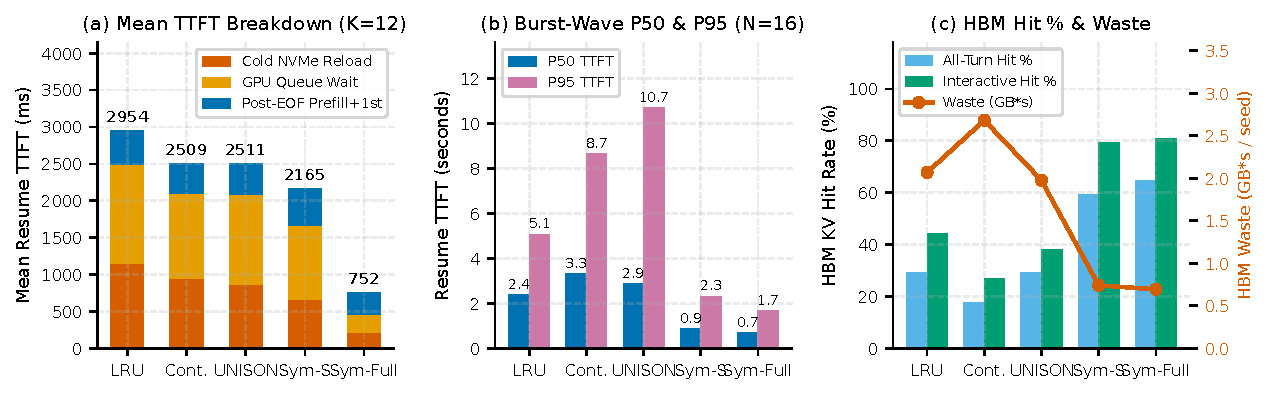
\includegraphics[width=0.98\textwidth]{fig2_phase0_ttft_decomposition.pdf}
\caption{Phase~0 real-hardware results on \texttt{Qwen2.5-3B-Instruct} ($1{,}080$ resumes across $3$ seeds). (a) Mean post-tool resume TTFT decomposition in the tight $290~\mathrm{MB}$ closed-pool regime ($K=12$), showing simultaneous reductions in cold NVMe reload wait, GPU queue wait, and post-exit prefill. (b) Median and P95 TTFT in the $16$-session burst wave ($380~\mathrm{MB}$). (c) Overall and interactive HBM KV hit rates alongside dead plus stalled HBM waste.}
\label{fig:phase0}
\end{figure*}

\subsection{Phase 0: Controlled Multi-Regime Analysis and Tandem Synergy}
Table~\ref{tab:phase0} and Fig.~\ref{fig:phase0} evaluate all five policies under two complementary load patterns on \texttt{Qwen2.5-3B-Instruct} ($B_{\mathrm{dma}} = 160~\mathrm{MB/s}$, equivalent to $1.6~\mathrm{GB/s}$ contended NVMe-to-PCIe bandwidth at $32\mathrm{B}$ KV scale): a closed concurrency pool ($K = 12$ active container slots draining $20$ two-turn episodes per seed, $M_{\mathrm{HBM}} = 290~\mathrm{MB}$) and a $16$-session concurrent burst wave ($M_{\mathrm{HBM}} = 380~\mathrm{MB}$).

Three empirical phenomena stand out. First, \Continuum{} suffers severe TTL cliff misses in both regimes ($15.8\%$ and $17.7\%$ overall HBM hit rates, dropping below reactive \texttt{LRU+CFS} at $18.3\%$ and $29.2\%$) because $3{:}1$--$4{:}1$ fair-share CPU contention stretches $2.0~\mathrm{s}$ \texttt{pytest} suites past $4.0$--$4.3~\mathrm{s}$ while disguised \texttt{stalled\_io} waits stay pinned in HBM across the entire TTL ($2{,}681.0~\mathrm{MB}\cdot\mathrm{s}$ waste in burst waves). Second, closing the OS-to-KV loop in \SymbioSched{} cuts burst-wave HBM waste by $2.8\times$--$3.6\times$ (to $739.8~\mathrm{MB}\cdot\mathrm{s}$), raises interactive hit rate from $27.0\%$--$44.4\%$ to $79.4\%$, and lowers median TTFT from $2{,}394$--$3{,}319~\mathrm{ms}$ to $888.5~\mathrm{ms}$.

Third, comparing \SymbioFull{} against \SymbioSched{} validates Theorem~\ref{thm:jit}(b)'s second-order tandem-queue coupling. In the tight $290~\mathrm{MB}$ closed-pool regime, Turn-2 KV caches grow to $82$--$92~\mathrm{MB}$; under \SymbioSched{}, three simultaneously exiting sessions occupy $255~\mathrm{MB}$ of HBM while waiting sequentially to prefill $1{,}050$ unstreamed \texttt{stdout} tokens, causing temporary HBM head-of-line backpressure ($\mathrm{P95} = 8{,}527~\mathrm{ms}$). By pre-encoding $89$ chunks of $256$ tokens during idle GPU slack, \SymbioFull{} drains waiting GPU sessions $1.7\times$ faster ($299.0~\mathrm{ms}$ vs.\ $505.0~\mathrm{ms}$ post-exit GPU service), cutting mean GPU queue wait by $4.2\times$ ($992.2 \to 235.5~\mathrm{ms}$), lifting HBM hit rate further from $42.5\%$ to $50.8\%$ ($59.4\% \to 64.6\%$ in burst waves), collapsing closed-pool P50 TTFT to $682.1~\mathrm{ms}$ ($3.6\times$--$3.7\times$ faster than baselines), raising raw cluster goodput from $34.89$ to $41.09~\mathrm{ep/min}$ ($+17.8\%$), and boosting strict $\le 500~\mathrm{ms}$ SLO goodput by $4.4\times$--$5.8\times$ ($32.9$ vs.\ $5.7$--$7.5~\mathrm{resumes/min}$).

\begin{table*}[!t]
\centering
\caption{Phase 1 Real Developer-Tool Process Groups (\texttt{pytest 9.2}, \texttt{clang++ -O3}, \texttt{git}) Across Three LLM Architectures ($K{=}10$, $C{=}3$ Cores)}
\label{tab:phase1}
\setlength{\tabcolsep}{4.6pt}
\begin{tabular}{llrrrrrrrrr}
\toprule
\textbf{Model Architecture} & \textbf{Policy} & \textbf{TTFT P50} & \textbf{TTFT P95} & \textbf{Cold Wait} & \textbf{EOF Prefill} & \textbf{HBM Hit} & \textbf{Inter.\ Hit} & \textbf{HBM Waste} & \textbf{Mean JCT} & \textbf{SLO Goodput} \\
\textbf{(\texttt{FP16} MPS)} & & \textbf{(ms)} & \textbf{(ms)} & \textbf{(ms)} & \textbf{(ms)} & \textbf{(\%)} & \textbf{(\%)} & \textbf{(MB$\cdot$s)} & \textbf{(s)} & \textbf{($\le 600$ms/m)} \\
\midrule
\multirow{5}{*}{\shortstack[l]{\texttt{Qwen2.5-3B}\\Dense GQA ($36$ KB/tok)\\$M_{\mathrm{HBM}}{=}320$MB}}
 & \texttt{LRU + CFS} & 1209.6 & 1973.2 & 444.2 & 242.7 & 43.8\% & 64.3\% & 2199.1 & 8.70 & 26.1 \\
 & \Continuum{} & 1265.7 & 2077.1 & 446.0 & 244.2 & 40.6\% & 59.5\% & 1649.3 & 8.95 & 22.2 \\
 & \UNISON{} & 1099.4 & 1800.3 & 287.6 & 249.1 & 54.7\% & 73.8\% & 1735.5 & 9.20 & 25.3 \\
 & \SymbioSched{} & 357.1 & 913.5 & \textbf{89.3} & 249.6 & \textbf{70.3\%} & \textbf{95.2\%} & 733.8 & 8.10 & 83.2 \\
 & \textbf{\SymbioFull{}} & \textbf{262.6} & \textbf{868.6} & 107.4 & \textbf{160.2} & 68.8\% & \textbf{95.2\%} & \textbf{695.5} & \textbf{7.97} & \textbf{90.4} \\
\midrule
\multirow{5}{*}{\shortstack[l]{\texttt{Qwen2.5-7B}\\Dense GQA ($56$ KB/tok)\\$M_{\mathrm{HBM}}{=}500$MB}}
 & \texttt{LRU + CFS} & 4355.2 & 7566.7 & 1301.8 & 578.1 & 26.6\% & 35.7\% & 2293.7 & 14.81 & 3.0 \\
 & \Continuum{} & 4064.3 & 6201.1 & 1053.8 & 550.8 & 23.4\% & 33.3\% & 2094.6 & 14.36 & 3.2 \\
 & \UNISON{} & 3918.0 & 5872.2 & 897.0 & 534.5 & 29.7\% & 42.9\% & 1765.3 & 14.43 & 2.1 \\
 & \SymbioSched{} & \textbf{1765.1} & \textbf{3552.4} & \textbf{248.6} & 528.3 & \textbf{54.7\%} & \textbf{81.0\%} & 1327.0 & 13.26 & 4.7 \\
 & \textbf{\SymbioFull{}} & 2210.5 & 3651.7 & 324.5 & \textbf{491.9} & 50.0\% & 76.2\% & \textbf{1323.4} & \textbf{12.67} & \textbf{8.4} \\
\midrule
\multirow{5}{*}{\shortstack[l]{\texttt{OLMoE-1B-7B}\\Sparse MoE ($128$ KB/tok)\\$M_{\mathrm{HBM}}{=}1140$MB}}
 & \texttt{LRU + CFS} & 2216.3 & 3004.1 & 569.4 & 353.2 & 32.8\% & 47.6\% & 7671.7 & 10.33 & 10.1 \\
 & \Continuum{} & 2021.5 & 2977.2 & 539.8 & 352.0 & 37.5\% & 54.8\% & 5641.4 & 10.24 & 10.2 \\
 & \UNISON{} & 2085.7 & 3124.0 & 504.9 & 350.8 & 39.1\% & 57.1\% & 5053.2 & 10.17 & 11.9 \\
 & \SymbioSched{} & 911.0 & \textbf{1494.6} & \textbf{114.9} & 352.9 & \textbf{67.2\%} & \textbf{90.5\%} & \textbf{2577.6} & 8.04 & 29.3 \\
 & \textbf{\SymbioFull{}} & \textbf{580.9} & 1651.6 & 137.2 & \textbf{280.3} & 64.1\% & 88.1\% & 2827.3 & \textbf{8.01} & \textbf{57.6} \\
\bottomrule
\end{tabular}
\end{table*}

\begin{figure*}[!t]
\centering
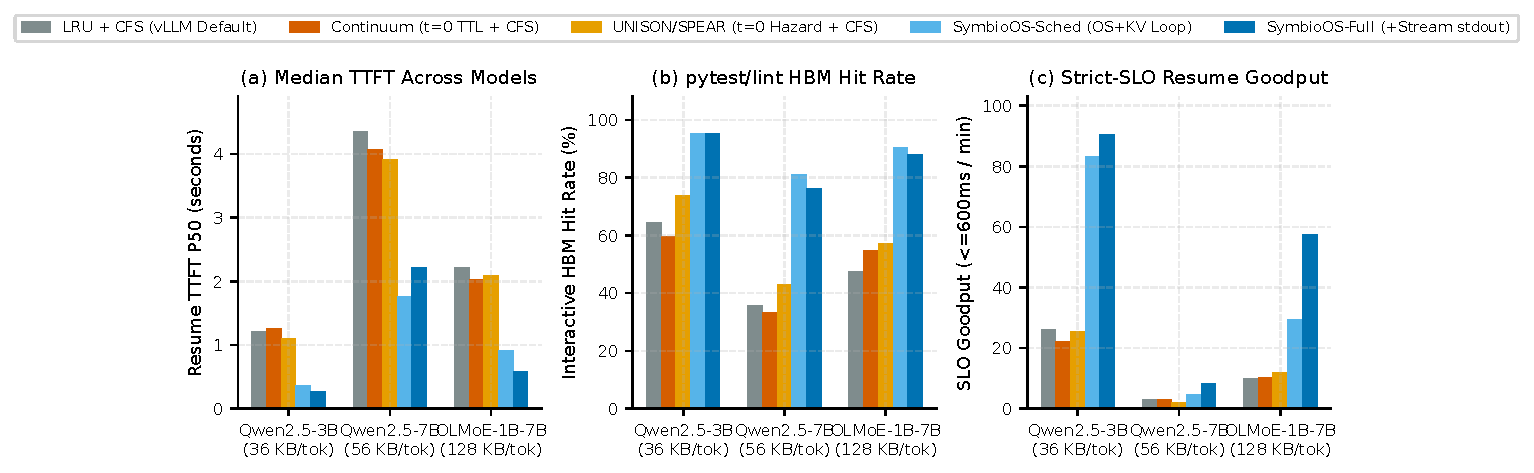
\includegraphics[width=0.98\textwidth]{fig3_multimodel_devtools.pdf}
\caption{Phase~1 multi-architecture evaluation across real \texttt{pytest~9.2}, \texttt{clang++ -O3 -c}, and \texttt{git} POSIX process groups (\texttt{os.killpg}). (a) Median post-tool resume TTFT, (b) interactive (\texttt{pytest}/\texttt{lint}) HBM KV hit rate, and (c) strict $\le 600~\mathrm{ms}$ SLO resume goodput across \texttt{Qwen2.5-3B}, \texttt{Qwen2.5-7B}, and sparse MoE \texttt{OLMoE-1B-7B}.}
\label{fig:multimodel}
\end{figure*}

\subsection{Phase 1: Real Developer Tools Across Three Model Architectures}
Table~\ref{tab:phase1} and Fig.~\ref{fig:multimodel} report real process-group scheduling (\texttt{os.killpg}) over genuine \texttt{pytest~9.2.0} suites ($20$ test cases across $5$ modules), multi-unit \texttt{clang++ -O3 -std=c++20 -c} C++ compilations ($8$--$9$ translation units), \texttt{py\_compile}/AST/\texttt{git} checks, and remote-socket fixture hangs across \texttt{Qwen2.5-3B}, \texttt{Qwen2.5-7B}, and \texttt{OLMoE-1B-7B} ($K = 10$ container slots, $C = 3$ CPU cores, proportional $M_{\mathrm{HBM}} \in \{320, 500, 1140\}~\mathrm{MB}$).

Across every model family, \SymbioOS{} delivers large, consistent gains:
\begin{itemize}
\item On \texttt{Qwen2.5-3B} ($36~\mathrm{KB/tok}$), \SymbioFull{} cuts median TTFT from $1{,}099.4$--$1{,}265.7~\mathrm{ms}$ down to $262.6~\mathrm{ms}$ ($4.19\times$--$4.82\times$ speedup), raises interactive \texttt{pytest}/\texttt{lint} HBM hit rate from $59.5\%$--$73.8\%$ to $95.2\%$, reduces HBM waste by $3.16\times$ versus \texttt{LRU+CFS}, and boosts $\le 600~\mathrm{ms}$ SLO goodput by $3.46\times$--$4.07\times$ ($90.4$ vs.\ $22.2$--$26.1~\mathrm{resumes/min}$).
\item On compute-heavy \texttt{Qwen2.5-7B} ($56~\mathrm{KB/tok}$), where single-GPU dense prefill utilizes $\approx 72\%$ of MPS capacity, \SymbioSched{} lowers median TTFT by $2.22\times$--$2.47\times$ ($3{,}918$--$4{,}355~\mathrm{ms} \to 1{,}765.1~\mathrm{ms}$) and lifts interactive HBM hit rate from $33.3\%$--$42.9\%$ to $81.0\%$, while \SymbioFull{} achieves the fastest mean episode JCT ($12.67~\mathrm{s}$ vs.\ $14.36$--$14.81~\mathrm{s}$), highest episode goodput ($38.55$ vs.\ $32.13~\mathrm{ep/min}$, $+20.0\%$), and $2.6\times$--$4.0\times$ higher SLO goodput ($8.4$ vs.\ $2.1$--$3.2~\mathrm{resumes/min}$).
\item On sparse MoE \texttt{OLMoE-1B-7B} ($128~\mathrm{KB/tok}$), fast $1\mathrm{B}$-active expert compute paired with $3.56\times$ larger MHA KV caches creates ideal conditions for both closed-loop tiering and idle-slack streaming: \SymbioFull{} slashes median TTFT by $3.48\times$--$3.82\times$ ($2{,}021.5$--$2{,}216.3~\mathrm{ms} \to 580.9~\mathrm{ms}$), raises interactive hit rate to $88.1\%$ ($90.5\%$ in \SymbioSched{}), cuts HBM waste from $7{,}671.7$ to $2{,}827.3~\mathrm{MB}\cdot\mathrm{s}$, lifts raw cluster goodput by $+21.6\%$ ($55.88$ vs.\ $45.95~\mathrm{ep/min}$), and increases strict-SLO goodput by $4.8\times$--$5.7\times$ ($57.6$ vs.\ $10.1$--$11.9~\mathrm{resumes/min}$).
\end{itemize}

\begin{table}[!t]
\centering
\caption{Per-Archetype Mechanism Dissection on \texttt{Qwen2.5-3B} (Real \texttt{pytest}, \texttt{clang++}, and \texttt{git} Process Groups)}
\label{tab:archetype}
\setlength{\tabcolsep}{3.4pt}
\begin{tabular}{llrrr}
\toprule
\textbf{Tool Class} & \textbf{Policy} & \textbf{Tool Wall (s)} & \textbf{HBM Hit (\%)} & \textbf{Mean TTFT (ms)} \\
\midrule
\multirow{3}{*}{\texttt{pytest\_suite}}
 & \texttt{LRU + CFS} & 2.14 & 50.0\% & 1048.5 \\
 & \Continuum{} & 2.30 & 43.3\% & 1177.0 \\
 & \textbf{\SymbioFull{}} & \textbf{1.93} & \textbf{93.3\%} & \textbf{248.0} \\
\midrule
\multirow{3}{*}{\texttt{heavy\_compile}}
 & \texttt{LRU + CFS} & 7.04 & 0.0\% & 1511.1 \\
 & \Continuum{} & \textbf{6.72} & 0.0\% & 1675.6 \\
 & \textbf{\SymbioFull{}} & 9.41 & \textbf{33.3\%} & \textbf{523.6} \\
\midrule
\multirow{3}{*}{\texttt{stalled\_io}}
 & \texttt{LRU + CFS} & 4.94 & 10.0\% & 1097.8 \\
 & \UNISON{} & 4.95 & 40.0\% & 879.1 \\
 & \textbf{\SymbioFull{}} & 5.38 & \textbf{0.0\%} & \textbf{504.8} \\
\bottomrule
\end{tabular}
\end{table}

\subsection{Per-Archetype Mechanism Dissection}
To verify how each closed-loop mechanism affects distinct workload classes rather than shifting tail latency onto background jobs, Table~\ref{tab:archetype} disaggregates Phase~1 \texttt{Qwen2.5-3B} results across \texttt{pytest\_suite}, \texttt{heavy\_compile}, and \texttt{stalled\_io} (all policies achieve $100\%$ HBM hit rate on $0.15~\mathrm{s}$ \texttt{quick\_lint} checks, where \SymbioFull{} still cuts mean TTFT from $904.1$--$1{,}002.7~\mathrm{ms}$ to $226.6~\mathrm{ms}$ by eliminating GPU queue backlog).

On interactive \texttt{pytest\_suite} runs, \SymbioFull{} prioritizes HBM-resident process groups so mean test wall-clock duration drops from $2.30~\mathrm{s}$ (\Continuum{}) to $1.93~\mathrm{s}$, raising HBM hit rate from $43.3\%$ to $93.3\%$ ($28/30$ suites) and cutting mean post-tool TTFT by $4.75\times$ ($1{,}177.0 \to 248.0~\mathrm{ms}$). On multi-file \texttt{clang++ -O3} builds (\texttt{heavy\_compile}), GPU-blind policies suffer $0.0\%$ HBM hit rates ($1{,}511.1$--$1{,}675.6~\mathrm{ms}$ TTFT) despite giving builds equal CPU share; \SymbioFull{} yields CPU quanta during early build phases ($9.41~\mathrm{s}$ wall time) and then triggers Theorem~\ref{thm:jit} JIT promotion once compiler milestones pass $[60\%]$--$[80\%]$, rescuing $33.3\%$ of build caches ($41.7\%$ in \SymbioSched{}) and cutting build-resume TTFT by $2.89\times$--$3.20\times$ (to $523.6~\mathrm{ms}$). Finally, on \texttt{stalled\_io} fixture waits, \UNISON{} retains $40.0\%$ of stalled caches in HBM due to $t = 0$ \texttt{pytest} label ambiguity, whereas \SymbioFull{} demotes $100\%$ of stalled caches at $1.25~\mathrm{s}$ ($0.0\%$ wasted exit residency) while still cutting post-recovery TTFT from $879.1$--$1{,}097.8~\mathrm{ms}$ to $504.8~\mathrm{ms}$.

\begin{figure*}[!t]
\centering
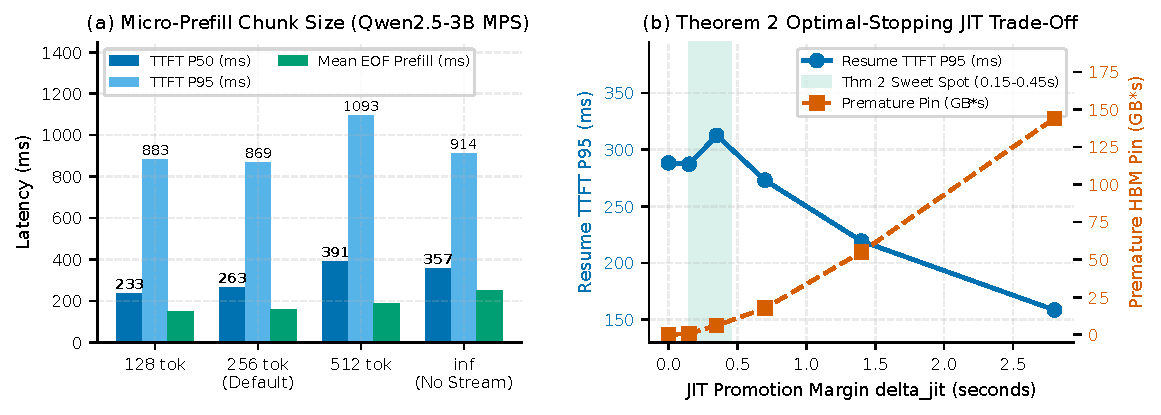
\includegraphics[width=0.90\textwidth]{fig4_chunk_and_jit_ablation.pdf}
\caption{Mechanism sensitivity studies. (a) Streaming \texttt{stdout} micro-prefill chunk-size sweep ($B_{\mathrm{chunk}} \in \{128, 256, 512, \infty\}$ tokens) on real \texttt{Qwen2.5-3B} MPS + \texttt{pytest} process groups. (b) Theorem~\ref{thm:jit} optimal-stopping JIT margin $\delta_{\mathrm{jit}}$ sweep at $N=128$, showing the trade-off between P95 resume TTFT and premature HBM pinning.}
\label{fig:ablation}
\end{figure*}

\subsection{Micro-Prefill Chunk Size and JIT Stopping Ablations}
Fig.~\ref{fig:ablation}(a) evaluates $B_{\mathrm{chunk}} \in \{128, 256, 512, \infty\}$ on \texttt{Qwen2.5-3B} with real \texttt{pytest} process groups. Disabling streaming ($B_{\mathrm{chunk}} = \infty$, \SymbioSched{}) leaves $249.6~\mathrm{ms}$ of mean post-exit prefill ($\mathrm{P50} = 357.1~\mathrm{ms}$, $\mathrm{P95} = 913.5~\mathrm{ms}$). Coarse $512$-token chunks capture fewer full blocks before tool exit ($23$ chunks) and occupy the GPU longer per non-preemptive step, raising P95 TTFT to $1{,}092.8~\mathrm{ms}$. Fine $128$-token chunks ($119$ chunks) achieve the lowest median TTFT ($233.2~\mathrm{ms}$) and fastest JCT ($7.88~\mathrm{s}$), whereas $256$-token chunks ($51$ chunks) achieve the lowest P95 tail latency ($868.6~\mathrm{ms}$) with minimal per-step dispatch overhead.

Fig.~\ref{fig:ablation}(b) sweeps the Theorem~\ref{thm:jit} JIT safety margin $\delta_{\mathrm{jit}} \in [0.0, 2.8]~\mathrm{s}$ at $N = 128$ sandboxes. Staging too late ($\delta_{\mathrm{jit}} = 0.0~\mathrm{s}$) incurs zero premature HBM pinning ($0.00~\mathrm{GB}\cdot\mathrm{s}$) at $68.1\%$ hit rate; overly aggressive staging ($\delta_{\mathrm{jit}} = 2.8~\mathrm{s}$) raises hit rate to $94.9\%$ at the cost of $144.11~\mathrm{GB}\cdot\mathrm{s}$ of premature HBM pinning. Operating in the critical-fractile band $\delta_{\mathrm{jit}} \in [0.15, 0.45]~\mathrm{s}$ captures timely promotions while bounding premature pinning below $6.1~\mathrm{GB}\cdot\mathrm{s}$ ($< 0.9\%$ of HBM budget).

\begin{table}[!t]
\centering
\caption{Phase 2 HBM Capacity Frontier at Cluster Scale ($N = 128$ Concurrent Sandboxes, $32\mathrm{B}/70\mathrm{B}$ KV Economics)}
\label{tab:scaleout}
\setlength{\tabcolsep}{3.6pt}
\begin{tabular}{rcccccc}
\toprule
\textbf{HBM} & \multicolumn{2}{c}{\textbf{TTFT P50 (ms)}} & \multicolumn{2}{c}{\textbf{HBM Hit (\%)}} & \multicolumn{2}{c}{\textbf{Goodput (ep/m)}} \\
\cmidrule(lr){2-3}\cmidrule(lr){4-5}\cmidrule(lr){6-7}
\textbf{Ratio} & \texttt{LRU} & \textbf{Sym-Full} & \texttt{LRU} & \textbf{Sym-Full} & \texttt{LRU} & \textbf{Sym-Full} \\
\midrule
15\% & 3701.9 & \textbf{638.1} & 23.6\% & \textbf{29.9\%} & 203.2 & \textbf{225.2} \\
25\% & 506.6 & \textbf{131.7} & 39.5\% & \textbf{49.7\%} & 203.6 & \textbf{217.9} \\
38\% & 59.4 & \textbf{40.2} & 60.2\% & \textbf{69.4\%} & 202.0 & \textbf{212.2} \\
50\% & 51.4 & \textbf{40.8} & 67.3\% & \textbf{77.6\%} & 202.0 & \textbf{212.6} \\
65\% & 40.1 & \textbf{38.9} & 77.6\% & \textbf{82.4\%} & 202.0 & \textbf{211.7} \\
\bottomrule
\end{tabular}
\end{table}

\begin{figure*}[!t]
\centering
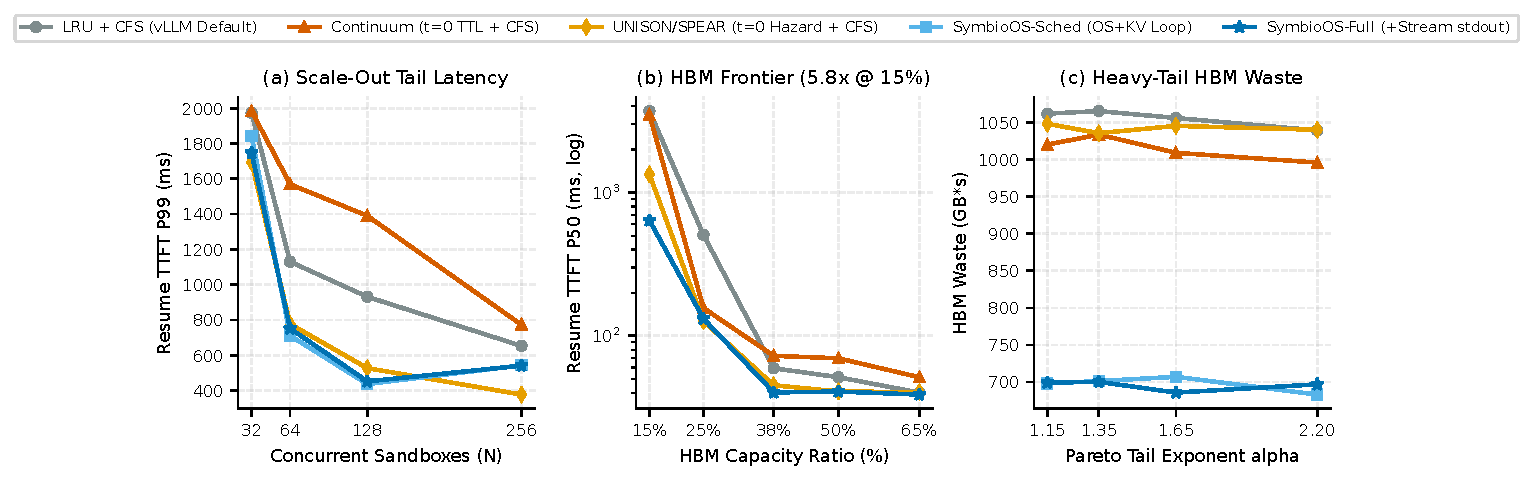
\includegraphics[width=0.98\textwidth]{fig5_cluster_scaleout_sweeps.pdf}
\caption{Phase~2 cluster-scale discrete-event tandem-queue sweeps ($32\mathrm{B}/70\mathrm{B}$ GQA KV footprint at $160~\mathrm{KB/tok}$). (a) Concurrency scale-out $N \in \{32, 64, 128, 256\}$ P99 resume TTFT. (b) Fast-HBM capacity ratio sweep ($15\%$--$65\%$ at $N=128$, log scale), demonstrating $5.80\times$ P50 speedup at $15\%$ HBM. (c) Pareto tail exponent $\alpha \in [1.15, 2.20]$ versus dead plus stalled HBM waste.}
\label{fig:scaleout}
\end{figure*}

\subsection{Phase 2: Cluster Scale-Out ($N = 32..256$) and Pareto Tails}
Table~\ref{tab:scaleout} and Fig.~\ref{fig:scaleout} evaluate cluster scale-out from $N = 32$ to $256$ concurrent sandboxes using our calibrated tandem-queue simulator ($160~\mathrm{KB/tok}$ $32\mathrm{B}/70\mathrm{B}$ GQA KV economics, $3.2~\mathrm{GB/s}$ contended DMA and $36\mathrm{K}~\mathrm{tok/s}$ prefill per $64$-sandbox GPU node). Across $N \in \{64, 128, 256\}$ in Fig.~\ref{fig:scaleout}(a), \SymbioOS{} cuts P99 resume TTFT by $2.0\times$--$3.1\times$ relative to \texttt{LRU+CFS} and \Continuum{} (e.g., $451.2~\mathrm{ms}$ vs.\ $931.1$ and $1{,}390.2~\mathrm{ms}$ at $N = 128$). Along the tight-memory frontier in Table~\ref{tab:scaleout} and Fig.~\ref{fig:scaleout}(b), \SymbioFull{} at $15\%$ HBM reduces P50 TTFT by $5.80\times$ ($3{,}701.9 \to 638.1~\mathrm{ms}$) and at $25\%$ HBM by $3.85\times$ ($506.6 \to 131.7~\mathrm{ms}$), allowing a cluster with $25\%$ HBM capacity under \SymbioFull{} to outperform \texttt{LRU+CFS} provisioned with $1.5\times$--$2\times$ more HBM. Finally, sweeping Pareto tail exponent $\alpha \in \{1.15, 1.35, 1.65, 2.20\}$ in Fig.~\ref{fig:scaleout}(c) confirms Theorem~\ref{thm:gittins}: across even extreme heavy tails ($\alpha = 1.15$, infinite variance), \SymbioOS{} reduces cluster HBM waste by $34\%$ ($1{,}062 \to 700~\mathrm{GB}\cdot\mathrm{s}$) compared to GPU-blind schedulers.

% ============================================================================
\section{Related Work}\label{sec:related}
% ============================================================================

\emph{Multi-Turn and Disaggregated KV Serving:} \texttt{vLLM}~\cite{kwon2023vllm} and \texttt{SGLang}~\cite{zheng2024sglang} manage paged and radix-tree KV blocks within GPU HBM, while \texttt{DistServe}~\cite{zhong2024distserve} and \texttt{Sarathi-Serve}~\cite{agrawal2024sarathi} reduce prefill-decode interference through phase disaggregation and fixed-size chunked prefill. Multi-tier KV engines including \texttt{CachedAttention}~\cite{gao2024cachedattention}, \texttt{Mooncake}~\cite{qin2025mooncake}, \texttt{LMCache}~\cite{cheng2025lmcache}, and \texttt{Strata}~\cite{xie2026strata} transfer KV slabs across HBM, host DRAM, and NVMe SSDs after requests reach the inference router, without inspecting active OS tool sandboxes or pre-encoding live tool pipe streams before process exit.

\emph{Agent-Aware KV Residency and Prediction:} \Continuum{}~\cite{li2025continuum} introduces program-level scheduling and scalar TTL pinning at tool launch ($t = 0$). \UNISON{}~\cite{he2026unison} pairs its \texttt{SPEAR} survival-penalty eviction policy with idle-window DMA tiering, \texttt{Lachesis}~\cite{yang2026lachesis} maps KV segments across HBM and high-bandwidth flash by predicted lifetime, \texttt{CacheScout}~\cite{zhang2026cachescout} learns workflow execution semantics online atop \texttt{vLLM}, and \texttt{PBKV}~\cite{zheng2026pbkv} predicts future agent invocations across dynamic graphs. All five frameworks treat tool pause duration as an exogenous black box predicted at $t = 0$; none ingest sub-turn \texttt{stdout} pipe progress, boost host CPU quanta to rescue hot HBM caches from contention-induced TTL cliffs, or overlap streaming \texttt{stdout} prefill during tool execution.

\emph{OS Scheduling for AI Sandboxes and Queueing Theory:} \texttt{AgentCgroup}~\cite{zheng2026agentcgroup} characterizes tool-call resource bursts in coding agents~\cite{yang2024sweagent,wang2025openhands} and applies Linux \texttt{sched\_ext} and \texttt{cgroup} controls for host CPU and memory isolation, without tracking GPU KV residency or reload cost. Classical Gittins index theory~\cite{gittins1979bandit,aalto2009gittins,scully2020gittins} and process-lifetime load balancing~\cite{harcholbalter1997exploiting} establish index optimality under DHR service distributions on single-station CPU servers. \SymbioOS{} bridges these two lines of work by coupling host POSIX quantum priority, optimal-stopping cold-tier DMA staging, and lookback-guarded BPE streaming~\cite{sennrich2016bpe} across a memory-coupled CPU-GPU tandem network~\cite{neely2010stochastic}.

% ============================================================================
\section{Discussion, Limitations, and Conclusion}\label{sec:conclusion}
% ============================================================================

\emph{Scope and Limitations:} First, \SymbioOS{} implements host CPU control in rootless user space via $80~\mathrm{ms}$ POSIX process-group quanta (\texttt{killpg}). While user-space signaling requires zero privileged capabilities and ports cleanly across Linux and macOS, sub-millisecond tool bursts shorter than one quantum experience coarse scheduling granularity; on bare-metal Linux 6.12+ hosts where root \texttt{CAP\_BPF} access is permitted, exporting our index \eqref{eq:impl_score} into a shared BPF map for \texttt{sched\_ext} or \texttt{cgroup v2} \texttt{cpu.weight} eliminates user-space signal ticks. Second, our hardware benchmarks run on a single $48~\mathrm{GB}$ Apple M5 Pro workstation with uncached SSD serialization (\texttt{F\_NOCACHE}) and single-GPU MPS execution; multi-node RDMA KV pools~\cite{qin2025mooncake} introduce cross-rack network jitter that should be incorporated into $T_{\mathrm{dma},i}$ when computing \eqref{eq:jit_thresh}. Third, opaque silent binaries that write zero progress bytes until termination fall back cleanly to command-class priors until $\sigma_i(t)$ crosses a conservative per-command silence threshold.

\emph{Conclusion:} Treating host OS sandbox scheduling and GPU KV memory tiering as independent problems causes severe TTL cliff evictions, stalled-cache HBM waste, and redundant post-exit prefill bottlenecks on multi-tenant coding-agent servers. \SymbioOS{} unifies rootless POSIX process-group scheduling, unstopped-quantum pipe filtration, KV-weighted Gittins CPU prioritization, optimal-stopping JIT promotion, and lookback-guarded $256$-token streaming \texttt{stdout} micro-prefill. Across $2{,}168$ real local tool-execution and MPS GPU resume cycles spanning \texttt{Qwen2.5-3B}, \texttt{Qwen2.5-7B}, and \texttt{OLMoE-1B-7B} alongside $256$-sandbox cluster simulations, \SymbioOS{} cuts median post-tool TTFT by up to $4.8\times$, lifts interactive HBM hit rates up to $95.2\%$, reduces HBM waste by up to $3.9\times$, and increases strict-SLO resume goodput by up to $5.7\times$.

\subsection*{Data and Code Availability}
The \SymbioOS{} runtime, rootless POSIX process-group sandbox drivers, multi-architecture benchmark harness, discrete-event tandem-queue simulator, raw JSON telemetry ($2{,}168$ hardware resumes and cluster sweeps), figure generation scripts, and LaTeX sources are available under Apache~2.0 at \url{https://github.com/batistado/symbioos}.

\subsection*{Acknowledgments and Competing Interests}
The authors declare no competing financial interests. All experiments executed locally using open-weight models on researcher hardware without external funding.

% ============================================================================
\appendices
\section{Formal Proofs}\label{app:proofs}
% ============================================================================

\begin{IEEEproof}[Proof of Proposition~\ref{prop:bpe}]
Let $\mathcal{P}: \Sigma^* \to (\Sigma^*)^*$ denote the regex pre-tokenizer of $\mathcal{T}$ (splitting raw text into non-overlapping lexical words/spans $w_1, w_2, \dots, w_K$ prior to BPE subword merges, which apply strictly inside each pre-token $w_r$~\cite{sennrich2016bpe}). Suppose $|\mathcal{T}(Y(t))| = n \ge 2$ with pre-tokens $w_1, \dots, w_K$ on $Y(t)$. Because $Y(t_{\mathrm{exit}}) = Y(t) \Vert Z$ appends bytes only at the right boundary of $w_K$, all completed pre-tokens $w_1, \dots, w_{K-1}$ are invariant under suffix concatenation $Z$, so their BPE merges match $\mathcal{T}(Y(t_{\mathrm{exit}}))$ identically. If $w_K$ encodes to $q \ge 2$ subwords, regex pre-tokenization boundaries ensure that once a multi-subword span or trailing delimiter has appeared, at most the final subword token $\mathcal{T}(Y(t))_n$ can merge with leading characters of $Z$; if $w_K$ encodes to $q = 1$ subword, dropping $\mathcal{T}(Y(t))_n$ removes all of $w_K$, leaving $\mathcal{T}(w_1 \cdots w_{K-1})$. In both cases, $\mathcal{T}_{\mathrm{safe}}(Y(t)) = \mathcal{T}(Y(t))_{1:n-1}$ is an exact prefix of $\mathcal{T}(Y(t_{\mathrm{exit}}))$.

For causal attention equivalence, let $X = [X_{\mathrm{pre}}; X_{\mathrm{pad}}] \in \mathcal{V}^B$ have $m \le B$ valid tokens starting at cache offset $L_0$. Because the causal mask enforces $M_{u,v} = -\infty$ for all key indices $v > L_0 + u$, for every query position $u \in \{1,\dots,m\}$ and layer $\ell \in \{1,\dots,L\}$, key-value projections $(K_{L_0+v}^{(\ell)}, V_{L_0+v}^{(\ell)})$ at padded indices $v > m$ receive exact zero softmax weight $\exp(-\infty) = 0$ and never enter the prefix reduction $\sum_{v=1}^{L_0+u} A_{u,v}^{(\ell)} V_v^{(\ell)}$. Cropping the final $B - m$ KV slots via $\mathrm{crop}(-(B - m))$ leaves identical cached tensors $(K_{1:L_0+m}^{(\ell)}, V_{1:L_0+m}^{(\ell)})$ and identical position-$(L_0+m)$ logits to an unpadded $m$-token step.
\end{IEEEproof}

\begin{IEEEproof}[Proof of Theorem~\ref{thm:gittins}]
Fix decision epoch $t$ with filtration $\mathcal{F}_t$ and conditional remaining CPU distribution $W_{\mathrm{rem},i} \mid \mathcal{F}_t$. In a single-server bandit allocation with holding/exposure reward $v_i$ collected upon completion of job $i$~\cite{gittins1979bandit,aalto2009gittins}, the classic Gittins index of job $i$ at attained service $u_i(t)$ is the supremum over positive stopping quanta $\Delta > 0$ of the expected reward-per-unit-time ratio:
\begin{equation}\label{eq:gittins_def}
\mathcal{G}_i(t) = \sup_{\Delta > 0} \frac{v_i\,\Prob\bigl(W_{\mathrm{rem},i} \le \Delta \mid \mathcal{F}_t\bigr)}{\E\bigl[\min(W_{\mathrm{rem},i},\, \Delta) \mid \mathcal{F}_t\bigr]}.
\end{equation}
Let $\bar{G}_i(x) = \Prob(W_{\mathrm{rem},i} > x \mid \mathcal{F}_t)$ with hazard $h_i(x) = g_i(x)/\bar{G}_i(x)$. Using $\E[\min(W_{\mathrm{rem},i}, \Delta) \mid \mathcal{F}_t] = \int_0^\Delta \bar{G}_i(x)\,\mathrm{d}x$ and $1 - \bar{G}_i(\Delta) = \int_0^\Delta h_i(x)\bar{G}_i(x)\,\mathrm{d}x$, the objective in \eqref{eq:gittins_def} is the weighted average of $v_i h_i(x)$ over $x \in [0, \Delta]$ with respect to density $\bar{G}_i(x) / \int_0^\Delta \bar{G}_i(y)\,\mathrm{d}y$. When $W_{\mathrm{rem},i} \mid \mathcal{F}_t$ is DHR ($h_i(x)$ non-increasing in $x$), for every $\Delta > 0$ we have
\begin{equation*}
\frac{\int_0^\Delta h_i(x)\bar{G}_i(x)\,\mathrm{d}x}{\int_0^\Delta \bar{G}_i(x)\,\mathrm{d}x} \ge \frac{\int_0^\infty h_i(x)\bar{G}_i(x)\,\mathrm{d}x}{\int_0^\infty \bar{G}_i(x)\,\mathrm{d}x} = \frac{1}{\E[W_{\mathrm{rem},i} \mid \mathcal{F}_t]},
\end{equation*}
and under scale-family DHR laws (such as Pareto $W_{\mathrm{rem},i} \sim \mathrm{Pareto}(\alpha, s_i(t))$ with $\alpha > 1$, or deterministic white-box milestone completion $W_{\mathrm{rem},i} = \hat{W}_{\mathrm{rem},i}(t)$ where $\Delta^* = \hat{W}_{\mathrm{rem},i}(t)$ achieves the supremum directly), $\mathcal{G}_i(t)$ is a strictly monotone constant multiple of $v_i / \E[W_{\mathrm{rem},i} \mid \mathcal{F}_t] = v_i / \E[R_i(t) \mid \mathcal{F}_t] = w_i(t)$. By Gittins' optimality theorem~\cite{gittins1979bandit,aalto2009gittins}, scheduling highest $\mathcal{G}_i(t)$ minimizes $\E[\sum_{i=1}^M v_i T_{\mathrm{wall},i}]$ for $C = 1$. For $C > 1$ identical cores, Scully et al.~\cite{scully2020gittins} prove via work-decomposition coupling against a single fast $C$-speed server that top-$C$ Gittins scheduling incurs excess weighted response bounded by $(C - 1)\max_i v_i$ times residual work, vanishing relative to total queue cost in heavy traffic.
\end{IEEEproof}

\begin{IEEEproof}[Proof of Theorem~\ref{thm:jit}]
For part~(a), expand the conditional expectation in \eqref{eq:jit_loss} with respect to $G_{i,t}(x) = \Prob(R_i(t) \le x \mid \mathcal{F}_t)$ evaluated around $T_d := T_{\mathrm{dma},i}$ (incorporating safety shift $\delta_{\mathrm{jit}} \ge 0$ via effective transfer window $\tilde{T}_d = T_d + \delta_{\mathrm{jit}}$):
\begin{equation*}
\mathcal{L}_i(t) = c_{\mathrm{miss}} \int_0^{\tilde{T}_d} (\tilde{T}_d - x)\,\mathrm{d}G_{i,t}(x) + \lambda_{\mathrm{hbm}} S_i \int_{\tilde{T}_d}^\infty (x - \tilde{T}_d)\,\mathrm{d}G_{i,t}(x).
\end{equation*}
Integrating by parts and taking the first-order variation with respect to delaying staging by an infinitesimal $\mathrm{d}t > 0$ (which shifts the residual distribution downward by $\mathrm{d}t$ under unit progress rate) gives marginal expected saving from staging now versus waiting:
\begin{equation*}
-\frac{\partial \mathcal{L}_i(t)}{\partial \tilde{T}_d} = -c_{\mathrm{miss}}\,G_{i,t}(\tilde{T}_d) + \lambda_{\mathrm{hbm}} S_i\bigl(1 - G_{i,t}(\tilde{T}_d)\bigr).
\end{equation*}
Staging strictly dominates waiting as soon as $c_{\mathrm{miss}} G_{i,t}(\tilde{T}_d) \ge \lambda_{\mathrm{hbm}} S_i (1 - G_{i,t}(\tilde{T}_d))$, which rearranges directly to $G_{i,t}(T_{\mathrm{dma},i} + \delta_{\mathrm{jit}}) \ge \frac{c_{\mathrm{miss}}}{c_{\mathrm{miss}} + \lambda_{\mathrm{hbm}} S_i} = 1 - \eta^*$. Because $R_i(t) \mid \mathcal{F}_t$ decreases stochastically in $t$ as $p_i(t) \uparrow 1$, $G_{i,t}(\tilde{T}_d)$ is non-decreasing, making the one-step lookahead rule optimal~\cite{neely2010stochastic}.

For part~(b), let $Q_1(k)$ denote the number of post-exit sessions queued at Station~1 at resume epoch $k$. Because streaming micro-prefill executes strictly when $Q_1 = 0$ in bounded chunks $B_{\mathrm{chunk}}/\mu_{\mathrm{pf}}$, any resume arriving to an empty GPU waits at most residual chunk time $\xi_{\mathrm{res}} \le B_{\mathrm{chunk}}/\mu_{\mathrm{pf}}$, while every post-exit service time shrinks from $\tau_{1,k}(0) = T_{\mathrm{cold},k} + L_{\mathrm{out},k}/\mu_{\mathrm{pf}} + \tau_{\mathrm{dec}}$ to $\tau_{1,k}(f_{\mathrm{stream}}) = T_{\mathrm{cold},k} + (1 - f_{\mathrm{stream}})L_{\mathrm{out},k}/\mu_{\mathrm{pf}} + \tau_{\mathrm{dec}}$ with $f_{\mathrm{stream}} > 0$. Applying the quadratic Lyapunov function $V(Q_1) = \frac{1}{2} Q_1^2$ over Station-1 service completions~\cite{neely2010stochastic} yields negative drift $\E[V(Q_1(k+1)) - V(Q_1(k)) \mid Q_1(k)] \le -Q_1(k)\bigl(1 - \lambda_{\mathrm{res}}\bar{\tau}_1(f_{\mathrm{stream}})\bigr) + O(1)$ whenever $\lambda_{\mathrm{res}}\bar{\tau}_1(f_{\mathrm{stream}}) < 1$, strictly containing $\lambda_{\mathrm{res}}\bar{\tau}_1(0) < 1$. By Pollaczek-Khinchine and Little's Law, smaller $\bar{\tau}_1$ and second moment $\E[\tau_1^2]$ strictly reduce $\E[W_{\mathrm{gpu}}]$ and pinned waiting HBM $\bar{M}_{\mathrm{wait}} = \lambda_{\mathrm{res}}\bar{S}\,\E[W_{\mathrm{gpu}}]$.
\end{IEEEproof}

\bibliographystyle{IEEEtran}
\bibliography{references}
\newpage

\begin{IEEEbiographynophoto}{Mohammed Kamran Syed}
received the M.S. degree in computer science. He is an IEEE Independent Researcher focusing on distributed inference systems, operating-system and GPU co-scheduling, KV-cache management, and fault-tolerant multi-agent orchestration.
\end{IEEEbiographynophoto}

\begin{IEEEbiographynophoto}{Anudeep Rentala}
is an IEEE Independent Researcher focusing on distributed systems, storage-compute disaggregation, and scalable inference runtimes for large language models.
\end{IEEEbiographynophoto}

\begin{IEEEbiographynophoto}{Somesh Rahul}
is an IEEE Independent Researcher working on runtime telemetry, cache consistency verification, and performance engineering for heterogeneous GPU clusters.
\end{IEEEbiographynophoto}

\begin{IEEEbiographynophoto}{Raghuram Malpe Pai}
is an IEEE Independent Researcher working on systems reliability, concurrency control, and deterministic workflow orchestration.
\end{IEEEbiographynophoto}

\begin{IEEEbiographynophoto}{Krishna Suman Dara}
is an IEEE Independent Researcher focusing on parallel architectures, distributed state synchronization, and machine learning systems infrastructure.
\end{IEEEbiographynophoto}

\end{document}
